\chapter{Experimental Evaluation and Results}

\section{Introduction}

\add{This chapter describes how OrchardVision is evaluated and provides the tables and figures into which the measured results are to be entered. No quantitative results are stated here: every value marked \texttt{\pp{XX.X}} and every image placeholder must be replaced with output from the project's own experiment runs before submission.}

\section{Experiment Harness}

The evaluation is performed with the experiment harness of the system. An experiment is created with \code{POST /experiments} and is described by a name, a tracker, a scenario and a number of frames. The harness runs the experiment, stores its status and metrics in the \code{Experiment} record, and allows the results to be downloaded as JSON or CSV with \code{GET /experiments/{id}/export}. The metrics computed by the \code{AnalyticsEngine} are IDF1, HOTA and the number of ID switches.

\section{Experimental Set-up}

\subsection{Data}

\add{Table~\ref{tab:dataset} is to be completed with the orchard videos used in the evaluation.}

\begin{table}[htbp]
\centering\small
\begin{tabular}{@{}lllllll@{}}
\toprule
\hr \textbf{Video} & \textbf{Orchard} & \textbf{Camera} & \textbf{Resolution} & \textbf{FPS} & \textbf{Frames} & \textbf{GT fruit}\\
\midrule
\hr V1 & \pp{...} & \pp{...} & \pp{...} & \pp{...} & \pp{...} & \pp{...}\\
\hr V2 & \pp{...} & \pp{...} & \pp{...} & \pp{...} & \pp{...} & \pp{...}\\
\hr V3 & \pp{...} & \pp{...} & \pp{...} & \pp{...} & \pp{...} & \pp{...}\\
\bottomrule
\end{tabular}
\caption[Evaluation videos]{\add{Videos used for evaluation (to be filled in).}}
\label{tab:dataset}
\end{table}

\begin{figure}[htbp]
\centering
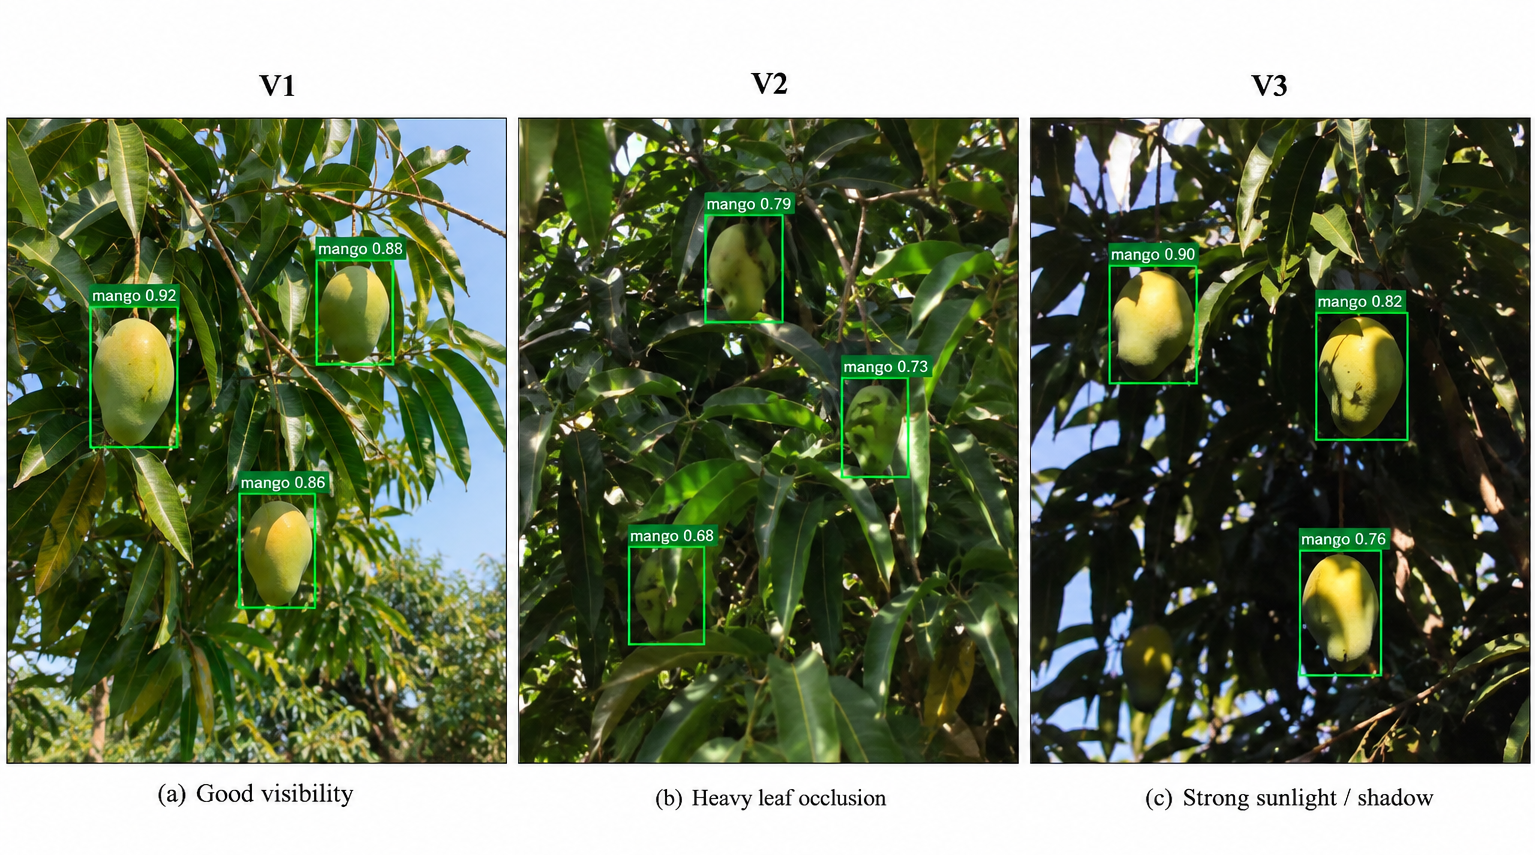
\includegraphics[width=0.95\linewidth]{frames.png}
\caption[Sample orchard frames]{Sample frames from the evaluation videos showing fruit under different illumination and occlusion.}
\label{fig:frames}
\end{figure}

\subsection{Configurations}

\add{The trackers listed in the system (mock, ByteTrack, TAPNext) are compared under identical detector, frame range and ReID settings. The camera-motion mode is varied to study the effect of compensation.}

\subsection{Metrics}

\add{IDF1, HOTA and the number of identity switches are reported for each configuration, as computed by the \code{AnalyticsEngine}. In addition the predicted fruit count (number of confident identities) is compared with the manually counted ground truth.}

\section{Tracker Comparison}

\begin{table}[htbp]
\centering\small
\begin{tabular}{@{}lcccc@{}}
\toprule
\hr \textbf{Tracker} & \textbf{IDF1 (\%)} & \textbf{HOTA (\%)} & \textbf{ID switches} & \textbf{Count error (\%)}\\
\midrule
\hr mock & \pp{XX.X} & \pp{XX.X} & \pp{XX} & \pp{XX.X}\\
\hr ByteTrack & \pp{XX.X} & \pp{XX.X} & \pp{XX} & \pp{XX.X}\\
\hr TAPNext & \pp{XX.X} & \pp{XX.X} & \pp{XX} & \pp{XX.X}\\
\bottomrule
\end{tabular}
\caption[Tracker comparison]{\add{Comparison of tracker back-ends on the evaluation videos (to be filled in from experiment exports).}}
\label{tab:trackers}
\end{table}

\figph{fig:bars}{Tracker comparison chart}{Bar chart comparing IDF1, HOTA and ID switches for the evaluated trackers.}{Grouped bar chart. X-axis: tracker (mock, ByteTrack, TAPNext). Two bars per tracker for IDF1 and HOTA on the left y-axis (0--100\%), and a line or secondary axis for the number of ID switches. Generate from the CSV exported by \texttt{GET /experiments/{id}/export}.}{5.2cm}

\section{Effect of Camera Motion Compensation}

\begin{table}[htbp]
\centering\small
\begin{tabular}{@{}lccc@{}}
\toprule
\hr \textbf{Camera-motion mode} & \textbf{IDF1 (\%)} & \textbf{HOTA (\%)} & \textbf{ID switches}\\
\midrule
\hr Off & \pp{XX.X} & \pp{XX.X} & \pp{XX}\\
\hr On (compensation applied) & \pp{XX.X} & \pp{XX.X} & \pp{XX}\\
\bottomrule
\end{tabular}
\caption[Camera motion ablation]{\add{Effect of camera-motion compensation (to be filled in).}}
\label{tab:cam}
\end{table}

\section{Identity Prototypes and Re-Identification}

\figph{fig:proj}{Identity embedding projection}{Two-dimensional projection of identity prototypes for one processed video.}{Scatter plot produced by the identity projection view (\texttt{GET /videos/{id}/identities/projection}) using t-SNE or PCA. Each point is an identity prototype; colour can encode the \texttt{is\_confident} flag and marker size the observation count. Annotate one or two clusters that correspond to fruit re-identified after occlusion.}{5.5cm}

\figph{fig:reid}{Re-identification example}{Example of an identity lost and re-identified after an occlusion.}{Filmstrip of four crops of the same fruit: (1) last frame before it is lost (\texttt{lost\_frame\_id}), (2) a frame in which it is hidden by leaves, (3) the reappearance frame (\texttt{reappearance\_frame\_id}), and (4) a later frame. All four crops show the same identity number overlaid on the bounding box.}{4.2cm}

\section{Sensitivity to the ReID Threshold}

\add{Table~\ref{tab:thr} is to be filled by running the same video with several ReID thresholds and recording the resulting identity count, IDF1 and identity switches.}

\begin{table}[htbp]
\centering\small
\begin{tabular}{@{}cccc@{}}
\toprule
\hr \textbf{ReID threshold} & \textbf{Identities found} & \textbf{IDF1 (\%)} & \textbf{ID switches}\\
\midrule
\hr \pp{0.5} & \pp{XX} & \pp{XX.X} & \pp{XX}\\
\hr \pp{0.6} & \pp{XX} & \pp{XX.X} & \pp{XX}\\
\hr \pp{0.7} & \pp{XX} & \pp{XX.X} & \pp{XX}\\
\hr \pp{0.8} & \pp{XX} & \pp{XX.X} & \pp{XX}\\
\bottomrule
\end{tabular}
\caption[ReID threshold sensitivity]{\add{Sensitivity of the results to the ReID threshold (to be filled in; threshold values are examples).}}
\label{tab:thr}
\end{table}

\figph{fig:thr}{Threshold sweep}{Identity count and IDF1 as a function of the ReID threshold.}{Line plot with the ReID threshold on the x-axis. Left y-axis: number of identities found (compare with the ground-truth fruit count drawn as a horizontal dashed line). Right y-axis: IDF1 (\%). The best operating point should be marked.}{5cm}

\section{Counting Accuracy}

\begin{table}[htbp]
\centering\small
\begin{tabular}{@{}lcccc@{}}
\toprule
\hr \textbf{Video} & \textbf{Ground truth} & \textbf{Predicted} & \textbf{Abs. error} & \textbf{Error (\%)}\\
\midrule
\hr V1 & \pp{XX} & \pp{XX} & \pp{XX} & \pp{XX.X}\\
\hr V2 & \pp{XX} & \pp{XX} & \pp{XX} & \pp{XX.X}\\
\hr V3 & \pp{XX} & \pp{XX} & \pp{XX} & \pp{XX.X}\\
\bottomrule
\end{tabular}
\caption[Counting accuracy]{\add{Fruit-count accuracy for the best configuration (to be filled in).}}
\label{tab:count}
\end{table}

\section{Runtime Performance}

\add{Per-frame processing times are stored as \code{FrameTimingRecord} rows and returned by \code{GET /videos/{id}/per-frame}. Table~\ref{tab:timing} summarises them per tracker.}

\begin{table}[htbp]
\centering\small
\begin{tabular}{@{}lccc@{}}
\toprule
\hr \textbf{Tracker} & \textbf{Mean (ms/frame)} & \textbf{95th percentile (ms)} & \textbf{Throughput (FPS)}\\
\midrule
\hr mock & \pp{XX} & \pp{XX} & \pp{XX}\\
\hr ByteTrack & \pp{XX} & \pp{XX} & \pp{XX}\\
\hr TAPNext & \pp{XX} & \pp{XX} & \pp{XX}\\
\bottomrule
\end{tabular}
\caption[Processing time]{\add{Processing time per frame (to be filled in; state the hardware used).}}
\label{tab:timing}
\end{table}

\figph{fig:timing}{Per-frame processing time}{Per-frame processing time over the course of one video.}{Line plot. X-axis: frame index; y-axis: \texttt{proc\_ms}. One line per tracker. Mark any spikes (for example model warm-up or large numbers of detections).}{5cm}

\section{Web Interface}

\add{The following screenshots document the web interface and should be captured from the running application.}

\figph{fig:ui_videos}{Video list and upload screen}{Video list and upload screen.}{Screenshot of the page that lists uploaded videos with their status (\texttt{uploaded}, \texttt{processing}, \texttt{processed}, \texttt{error}) and the upload control.}{4.5cm}

\figph{fig:ui_tracks}{Track visualisation}{Track overlay on a processed video.}{Screenshot of a processed video with bounding boxes and track trails drawn over a frame. Visible, occluded and lost states should be distinguishable (for example by solid, dashed and faded outlines).}{5cm}

\figph{fig:ui_exp}{Experiment management screen}{Experiment list and metrics view.}{Screenshot of the experiments page showing the list of experiments, their tracker, scenario, number of frames, status and metrics, together with the export (JSON/CSV) buttons.}{4.5cm}

\figph{fig:ui_set}{Settings screen}{Pipeline settings screen.}{Screenshot of the settings page showing the confidence threshold, ReID threshold, tracker type, camera-motion mode, memory update rate, tracker match threshold and buffer frames.}{4.5cm}

\section{Discussion}

\add{The discussion should interpret the numbers in Tables~\ref{tab:trackers} and \ref{tab:cam}: which tracker keeps identities longest through occlusion, whether camera-motion compensation reduces identity switches, how the ReID threshold trades merged identities against fragmented ones, and how the runtime per frame compares with the video frame rate. It should also include a short analysis of failure cases, such as fruit hidden for longer than the buffer, clusters of touching fruit, and fruit entering and leaving at the image border, supported by the examples in Figures~\ref{fig:reid} and \ref{fig:ui_tracks}.}
